\section{Trigonometrische Funktionen}
%
%
%
\subsubsection{Definition:}
$\alpha = R_{c,s}$ definiere $c=\cos \alpha, \, s=\sin\alpha, \, \frac{s}{c}=\tan\alpha$  sofern $c \neq 0$
%
 \begin{figure}[H]
 \centering
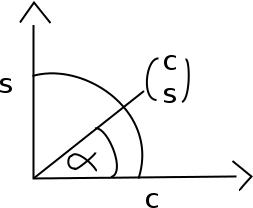
\includegraphics[width=0.15\textwidth]{mainmatter/chapter1/pics/trigo1.png}
\end{figure}
%
\qquad\\
 \begin{tabular}{|c|c|c|c|c|c|c|}
 \hline
Winkel & $0^{\circ}$ & $30^{\circ}$ & $45^{\circ}$ & $60^{\circ}$ & $90^{\circ}$ & $180^{\circ}$\\\hline
$\sin$ & 0 & $\frac{1}{2}$ & $\frac{1}{2}\sqrt{2}$ & $\frac{1}{2} \sqrt{3}$ & 1 & 0\\\hline
$\cos$ & 1 & $\frac{1}{2} \sqrt{3}$ &$\frac{1}{2}\sqrt{2}$ &  $\frac{1}{2}$  & 0 & -1\\\hline
$\tan$ & 0 &$\frac{1}{3}\sqrt{3}$ & 1 & $\sqrt{3}$ & - & 0 \\\hline
 \end{tabular}\\
 \qquad\\
 z.B. $45^{\circ} \, R_{c,s}$ mit $c=s$ \\
$R^{2}_{c,s} = \begin{pmatrix} \frac{1}{2}\sqrt{2} & - \frac{1}{2}\sqrt{2} \\ \frac{1}{2}\sqrt{2} & \frac{1}{2}\sqrt{2} \end{pmatrix}\begin{pmatrix} \frac{1}{2}\sqrt{2} & - \frac{1}{2}\sqrt{2} \\ \frac{1}{2}\sqrt{2} & \frac{1}{2}\sqrt{2} \end{pmatrix} = R_{0,1}= 90^{\circ} \Rightarrow R_{c,s} = 45^{\circ}$ \\
\qquad\\
 in allgemeiner Form:\\
 $ R^{2}_{c,s} = R_{c^{2}-s^{2},2cs}=R_{0,1}$\\
 \qquad\\
 analog $ c= \frac{1}{2}\sqrt{3}$ \\
 $s=\frac{1}{2}$\\
 $(R_{c,s})^{3} = R_{0,1}$ (nachrechnen !): $R_{c,s}^{3} = \begin{pmatrix} \frac{1}{2} & -\frac{1}{2}\sqrt{3} \\ \frac{1}{2}\sqrt{3} & \frac{1}{2} \end{pmatrix}\begin{pmatrix} \frac{1}{2}\sqrt{3} & -\frac{1}{2} \\ \frac{1}{2} & \frac{1}{2}\sqrt{3} \end{pmatrix} = \begin{pmatrix} 0 & -1 \\ 1 & 0 \end{pmatrix}$
 %
 %
 %
 \subsubsection{Satz:}
 $\cos^{2}\alpha + \sin^{2}\alpha =1$\\
 $\cos -\alpha=\cos\alpha, \, \sin\ -\alpha=-\sin\alpha$
 %
 %
%
 \subsubsection{Beweis:}
 $\alpha = R_{c,s} \, \cos^{2}\alpha+\sin^{2}\alpha= c^{2}+s^{2}=1$\\
 $-\alpha=R_{\mathop{c}\limits_{\mathop{\cos-\alpha = \cos \alpha}\limits^{\uparrow}}, \, \mathop{-s}\limits_{\mathop{\sin-\alpha = -\sin\alpha}\limits^{\uparrow}}}$\\
 %
 %
 %
 \subsubsection{Additionstheoreme:}
 \begin{enumerate}
 	\item $\cos(\alpha+\beta) = \cos\alpha\cdot\cos\beta-\sin\alpha\sin\beta$
 	\item $\sin(\alpha+\beta)=\sin\alpha\cos\beta+\cos\alpha\sin\beta$
\end{enumerate}
%
%
%
\subsubsection{Beweis:}
$\alpha=R_{c,s}$\\
$\beta=R_{t,u}$\\
$\alpha+\beta=R_{\mathop{\underbrace{ct-su}}\limits_{1.},\, \mathop{\underbrace{cu+st}}\limits_{2.}}$
%
%
%
\subsubsection{Satz:}
\begin{enumerate}
	\item $ <\vec{a},\vec{b}>=\cos(\measuredangle(a,b))\cdot\Vert\vec{a}\Vert
	\cdot\Vert\vec{b}\Vert$
	\item $det(\vec{a},\vec{b})=\sin(\measuredangle(a,b))\cdot\Vert\vec{a}\Vert
	\cdot \Vert\vec{b}\Vert$
\end{enumerate}
Für Vektoren der Länge 1 ist das Skalarprodukt der Cosinus und die Determinante der Sinus des eingeschlossenen Winkels. 
%
%
%
\subsubsection{Beweis:}
$\frac{\vec{a}}{\Vert\vec{a}\Vert}=\begin{pmatrix} c \\ s \end{pmatrix} \quad \frac{\vec{b}}{\Vert\vec{b}\Vert} = \begin{pmatrix} t \\ u \end{pmatrix} \quad \measuredangle(\vec{a},\vec{b})=R_{t,u}\cdot R_{c,-s}=R_{ct+su,uc-st}$\\
$\cos\measuredangle(a,b)=ct+su=\frac{<a,b>}{\Vert a \Vert \cdot \Vert b\Vert}$\\
$\sin\measuredangle(a,b)=uc-ts=\frac{det(\vec{a},\vec{b})}{\Vert\vec{a}\Vert\cdot\Vert\vec{b}\Vert}$
%
%
%
\subsubsection{Beispiel:}
\begin{enumerate}
	\item $\vec{a}\begin{pmatrix}2\\3\end{pmatrix} \, \vec{b}=
	\begin{pmatrix}-4\\1\end{pmatrix}$ \\
	$<\vec{a},\vec{b}>=-5\Rightarrow\cos\measuredangle(a,b)=\frac{-5}
	{\sqrt{13}\cdot\sqrt{17}} \mathop{\Rightarrow}\limits^{\text{TR}}\measuredangle
	(\vec{a},\vec{b})\approx110^{\circ}$
	\item $\vec{a}=\begin{pmatrix} 3 \\ 1 \end{pmatrix}, \, \vec{b}=\begin{pmatrix}2 \\ 4 
	\end{pmatrix}$\\
	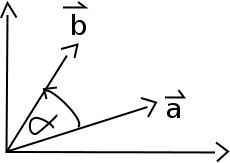
\includegraphics[width=0.15\textwidth]{mainmatter/chapter1/pics/trigo2.png}
	$
	\left.
	\begin{array}{cc}
	<a,b>=10 \\
	det(\vec{a},\vec{b})=10
	\end{array}
	\right\} 
	\Rightarrow \sin\alpha=\cos\alpha \Rightarrow \alpha = 45^{\circ}$
\end{enumerate}
%
%
%
\subsubsection{Satz:}	
$\vec{a} \neq \vec{0} \neq \vec{b} \qquad \measuredangle(\vec{a},\vec{b}-\vec{a})=\frac{\pi}{2}$. Dann gilt:\\

\begin{figure}[htbp]
	\begin{minipage}[t]{0.4\textwidth} 
	\begin{enumerate}
	\item $\cos \measuredangle(\vec{a},\vec{b})=\frac{\Vert\vec{a}\Vert}
	{\Vert\vec{b}\Vert} \qquad \frac{\textrm{Ankathete}}{\textrm{Hypotenuse}}$
	\item $\sin\measuredangle(\vec{a},\vec{b})=\pm\frac{\Vert\vec{b}-\vec{a}\Vert}
	{\Vert\vec{b}\Vert} \qquad \frac{\textrm{Gegenkathete}}{\textrm{Hypotenuse}}$
	\end{enumerate}
	\end{minipage}
	\begin{minipage}[b]{0.4\textwidth}
	\begin{figure}[H]
	\centering 
	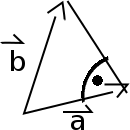
\includegraphics[width=0.3\textwidth]{mainmatter/chapter1/pics/trigo3.png}
	\end{figure}
	\end{minipage}
\end{figure}
%
\subsubsection{Beweis:}
\begin{enumerate}
	\item $0=<\vec{a},\vec{b}-\vec{a}>=<a,b>-<a,a>$\\
	$\Vert\vec{a}\Vert^{2}=<\vec{a},\vec{a}>=<\vec{a},\vec{b}>=
	\Vert\vec{a}\Vert\cdot\Vert\vec{b}\Vert\cdot(\cos\measuredangle(\vec{a},
	\vec{b}))$
	\item $\sin\alpha=\pm\sqrt{1-\cos^{2}\alpha}$\
		$\mathop{=}^{\text{1.}}\sqrt{\frac{\Vert\vec{b}\Vert^{2}-\Vert a \Vert^{2}}
		{\Vert b \Vert^{2}}} =\pm \frac{\Vert b-a\Vert}{-\Vert b \Vert}$ \qquad 	
		$\square$
\end{enumerate}
